\noindent The $\pi$ and T-type attenuators owe their names because to the shape of their layout. Both topologies are easy to implement, provide two-port matching and have broadband response. For these reasons, they are widely used in RF circuit design.

  \begin{figure}[ht]
    \centering
    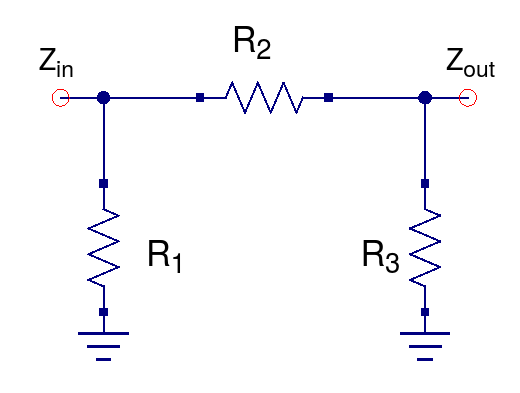
\includegraphics[width=5cm]{./images/pi-attenuator-schematic.png}
    \caption{$\pi$-type attenuator schematic}
    \label{fig:pi-type-attenuator-schematic}
  \end{figure}
  
\noindent The design equations are the following \cite{vizmuller1995rf}:

\begin{equation}
	R_2 = \frac{1}{2} \cdot (10^{\frac{\alpha}{10}} - 1) \cdot \sqrt{\frac{Z_{in} \cdot Z_{out}}{10^{\frac{\alpha}{10}}}}
\end{equation}

\begin{equation}
	R_1 = \frac{1} {\frac{10^{\frac{\alpha}{10}}+1}{Z_{in} \cdot (10^{\frac{\alpha}{10}} - 1)} - \frac{1}{R_2}}
\end{equation}

\begin{equation}
	R_3 = \frac{1} {\frac{10^{\frac{\alpha}{10}}+1}{Z_{out} \cdot (10^{\frac{\alpha}{10}} - 1)} - \frac{1}{R_2}}
\end{equation}


\noindent where $\alpha$ is the attenuation in dB. In both T- and $\pi$-type attenuator topologies the minumum attenuation possible depends on the input impedance $Z_{in}$ and the output impedance $Z_{out}$, as shown in Eq. \ref{eq:min_att_pi}

\begin{equation}
	\alpha_{min} = 20 \cdot log_{10} \left( \sqrt{\frac{Z_{in}}{Z_{out}}} + \sqrt{\frac{Z_{in}}{Z_{out}}-1} \right)
	\label{eq:min_att_pi}
\end{equation}


\noindent Fig. \ref{fig:tee-type-minimum-attenuation} shows the minimum attenuation possible in $\pi$ and T-type attenuators for $Z_{in} / Z_{out}$ ratios up to 10.
  
  \begin{figure}[H]
    \centering
    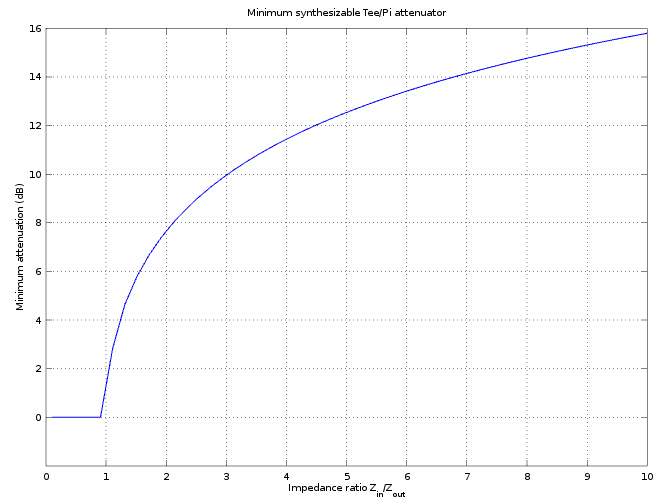
\includegraphics[width=10cm]{./images/pi-tee-minimum-attenuation-vs-Zin-Zout.png}
    \caption{Minimum attenuation possible in T and $\pi$-type attenuators}
    \label{fig:tee-type-minimum-attenuation}
  \end{figure}  

\noindent The power dissipated in each resistor can be derived using network analysis. Consider the voltages and currents in Fig. \ref{fig:power-dissipation-pi-type-attenuator} and let $P_{R1}$, $P_{R2}$ and $P_{R3}$ be the power dissipated by $R_1$, $R_2$ and $R_3$ respectively. Then: 

  \begin{figure}[H]
    \centering
    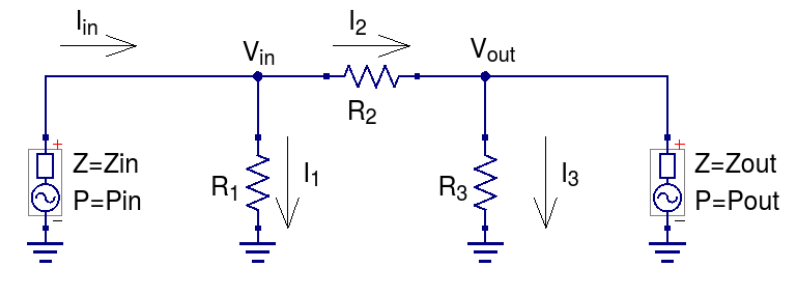
\includegraphics[width=10cm]{./images/pi-attenuator-power-dissipation.png}
    \caption{$\pi$-type attenuator schematic}
    \label{fig:power-dissipation-pi-type-attenuator}
  \end{figure}
  
  \begin{equation}
  	P_{R1} = P_{in} \cdot \frac{Z_{in}}{R_1}
  \end{equation}
  
  \begin{equation}
  	P_{R2} = P_{in} \cdot  \frac{R_2 \cdot (R_1 - Z_{in})^2}{R_1^2 \cdot Z_{in}}
  \end{equation}
   
  \begin{equation}
  	P_{R3} = P_{in} \cdot \frac{\left( R_1 \cdot R_2 - Z_{in} \cdot (R_1 + R_2) \right)^2}{R_1^2 \cdot R_3 \cdot Z_{in}}
  \end{equation}